\documentclass[12pt,letterpaper]{article}
\usepackage[margin=1in,headheight=15pt]{geometry}
\usepackage{amsmath,amsthm}
\usepackage{newtxtext,newtxmath}
\usepackage{booktabs,array,microtype,fancyhdr,caption}
\usepackage{pgfplots}\pgfplotsset{compat=1.18}
\usetikzlibrary{arrows.meta,positioning,calc}
\usepackage[hidelinks]{hyperref}
\definecolor{main}{HTML}{0072B2}\definecolor{accent}{HTML}{D55E00}
\definecolor{green}{HTML}{009E73}
\pagestyle{fancy}\fancyhf{}\fancyhead[L]{Team 7391857}\fancyhead[R]{Merge After Toll}\fancyfoot[C]{\thepage}
\setlength{\parindent}{1.2em}\setlength{\parskip}{3pt}
\captionsetup{font=small,labelfont=bf}
\newtheorem{proposition}{Proposition}
\begin{document}
\thispagestyle{empty}
\noindent\begin{tabular*}{\textwidth}{@{\extracolsep{\fill}}lcr}
Problem Chosen & 2017 MCM & Team Control Number\\
\Large B & \Large Summary Sheet & \Large 7391857
\end{tabular*}
\vspace{1.0em}
\begin{center}{\LARGE\bfseries Paying for the Bottleneck:\\[4pt] A Compatible-Flow Design for Toll-Plaza Merging}\end{center}

We examine a barrier with 8 booths feeding 3 travel lanes. A first capacity calculation compares aggregate toll service with the exit lanes. It gives 5,400 vehicles/hour, but a separate payment-compatibility check limits the same arrangement to 3,000 vehicles/hour. Thus the pooled result cannot be used as a feasible operating recommendation.
A smooth fan-in connects each contiguous group of booths to an exit lane. Quintic lateral paths provide zero lateral velocity and acceleration at each end. Their maximum slope and acceleration determine a conditional minimum length. An exit headway rule separates successive discharges; it does not estimate crash frequency or model interactions inside the taper.
At light demand (1,200 vehicles/hour), average service capacity exceeds demand under the nominal payment mix. At heavy demand (3,600 vehicles/hour), staffed booths overload. Increasing automated-vehicle penetration can reduce exit headways, but cannot increase staffed-booth service. The next decision is therefore the number and assignment of payment-compatible booths, rather than simply a shorter taper or faster exit.
This baseline identifies the limiting mechanism but does not yet establish the best layout, finite-horizon delay or a design robust to payment shifts. The design recommendation is conditional: retain the smooth geometric concept, avoid treating pooled capacity as achievable, and resolve the payment allocation before selecting a construction option.
\noindent\textbf{Keywords:} toll plaza; compatible flow; minimum cut; queueing; geometric design.
\clearpage\tableofcontents\clearpage
\section{The design question}
The task is to design the departure side of a barrier toll, including its shape, dimensions and merging pattern, while balancing traffic throughput, accident prevention and construction cost \cite{comap}. We retain a general model with $B$ booths and $L<B$ exit lanes and examine the problem\'s eight-to-three example. Payment type and vehicle automation are different attributes: electronic toll collection does not imply an autonomous vehicle.
A useful design must explain why it improves on a plausible alternative. Our baseline uses a block of staffed booths, a block of exact-change booths and a block of electronic booths. Our proposed alternative distributes compatible service among channelized exit groups and controls release by the receiving lane. No claim of superiority over every existing real plaza is possible without local demand, geometry and compliance data.
\begin{table}[htbp]\centering\small\caption{How the requested decisions are answered.}\begin{tabular}{@{}p{.32\linewidth}p{.61\linewidth}@{}}\toprule
Decision & Model or evidence\\\midrule
Shape, size and pattern & Smooth fan-in and contiguous exit groups\\
Throughput and payment proportions & Compatible-flow network and cut threshold\\
Accident prevention & Kinematic bounds and controlled discharge\\
Cost & Pavement and equipment scenario; frontier\\
Light/heavy demand & Capacity screening; delay not yet quantified\\
Automated vehicles & Headway sensitivity with unchanged toll service\\
\bottomrule\end{tabular}\end{table}
\section{Inputs, assumptions and scope}
No site observations are supplied. Table~\ref{tab:inputs} defines transparent design scenarios; none of its numerical service, cost or behavior inputs is presented as a measured New Jersey value. The official problem provides the task, while FHWA guidance motivates distinguishing model verification from field calibration \cite{fhwa}. We do not calibrate a traffic model by choosing parameters that make our design look favorable.
\begin{table}[htbp]\centering\small\caption{Scenario inputs and their status.}\label{tab:inputs}\begin{tabular}{@{}p{.34\linewidth}p{.25\linewidth}p{.32\linewidth}@{}}\toprule
Input & Value & Interpretation\\\midrule
Booths / exit lanes & 8 / 3 & Worked design\\
Mean service: staffed / exact / ETC & 12.0 / 6.0 / 2.0 s & Assumed service scenarios\\
Service coefficients of variation & 0.50 / 0.30 / 0.10 & Lognormal service draws\\
Human / AV--AV headway & 2.0 / 0.9 s & Assumed exit control\\
Travel-lane width & 3.5 m & Geometric assumption\\
Booth center spacing & 3.5 m & Includes assumed island allowance\\
Departure speed & 10.0 m/s & Constant-speed path calculation\\
Maximum slope / lateral acceleration & 0.10 / 0.5 m/s$^2$ & Scenario constraints\\
Road construction & \$200 /m$^2$ & Cost scenario; excludes land purchase\\
Demand: light / heavy & 1,200 / 3,600 veh/h & 30-minute demand episodes\\
\bottomrule\end{tabular}\end{table}
Vehicles retain their payment class during a visit. Within each class, signs or advance assignment direct vehicles to compatible booths. Booths assigned to an exit group form a contiguous block, and vehicles do not cross group boundaries after payment. We assume adequate approach capacity and holding space when deriving the network threshold; queues in the simulation can wait without blocking upstream booths. These assumptions separate capacity screening from a fully resolved road simulation.
\begin{table}[htbp]\centering\small\caption{Demand proportions, independent of booth proportions.}\begin{tabular}{@{}lrrr@{}}\toprule
Scenario & Staffed & Exact & ETC\\\midrule
nominal & 30\% & 30\% & 40\%\\
cash heavy & 45\% & 35\% & 20\%\\
electronic heavy & 10\% & 15\% & 75\%\\
\bottomrule\end{tabular}\end{table}
Let $n_{gt}$ be the number of booths of payment type $t$ assigned to exit group $g$, $\mu_t=3600/s_t$ the mean booth service rate in vehicles/hour, and $p_t$ the proportion of arriving vehicles requiring type $t$. The arrival rate is $\lambda$; $C_g$ is the discharge capacity of exit $g$. A layout satisfies $n_{gt}\in\mathbb Z_{\ge0}$, $\sum_{g,t}n_{gt}=B$, and every exit group and payment class is nonempty in the worked search.
\section{Why aggregate capacity is not a design}
A pooled estimate is the upper bound $U=\min(\sum_{g,t}n_{gt}\mu_t,\sum_g C_g)$. It ignores whether the arriving drivers can use the available service. Every payment class separately requires $\lambda p_t\le\mu_t\sum_g n_{gt}$.
The baseline has booth totals 3/3/2. Its pooled bound is 5,400 vehicles/hour, whereas the payment bound is 3,000 vehicles/hour. In particular, staffed service supplies 900 vehicles/hour, which must serve 30\% of arrivals. Extra unused electronic capacity does not serve that queue.
This is one structural failure, not several unrelated numerical errors. It changes the throughput claim, the heavy-traffic interpretation and the preferred booth mix. A design based only on the pooled number would therefore need to be revised in all three places.
\section{A compatible-flow capacity certificate}
For a specified layout, let $x_{gt}$ be the rate of type-$t$ vehicles sent through group $g$. Feasible routing satisfies
\begin{align}
0\le x_{gt}&\le n_{gt}\mu_t, &\sum_g x_{gt}&=\lambda p_t, &\sum_t x_{gt}&\le C_g. \label{eq:flow}
\end{align}
Construct a directed network with source-to-type arcs of capacity $\lambda p_t$, type-to-group arcs $n_{gt}\mu_t$, and group-to-sink arcs $C_g$. The constraints hold exactly when the maximum flow equals $\lambda$. This representation preserves both payment compatibility and lane capacity.
\begin{proposition}
For $p_t>0$, the largest feasible fluid rate in this network is
\begin{equation}
\lambda^*(n,p,C)=\min_{\varnothing\ne S\subseteq\{1,\ldots,T\}}
\frac{\sum_g\min\{C_g,\sum_{t\in S}n_{gt}\mu_t\}}{\sum_{t\in S}p_t}.\label{eq:cut}
\end{equation}
\end{proposition}
\begin{proof}
Fix the set $S$ of type nodes on the source side of a cut. The source arcs of all other types contribute $\lambda(1-p(S))$. For each group, placing it on the sink side cuts the type-to-group arcs from $S$, while placing it on the source side cuts its exit arc. The least contribution is therefore $\min(C_g,\sum_{t\in S}n_{gt}\mu_t)$. Every cut has capacity at least $\lambda$ precisely when the inequalities in \eqref{eq:cut} hold. The empty set imposes no restriction. The maximum-flow/minimum-cut theorem then gives sufficiency as well as necessity.
\end{proof}
With three payment classes, only seven reduced cuts are needed per layout. A linear program constructs the rates $x_{gt}$ after selection; it is not used to manufacture an optimum claim. Equation~\eqref{eq:cut} is a fluid capacity threshold. Under variable arrivals and service, equality is not a finite-delay operating guarantee: steady operation needs slack, and finite peak episodes can exceed capacity while accumulating queues.
The certificate gives a route to improve the baseline, but this draft does not yet enumerate layouts or quantify queue delays. It supports the rejection of the pooled recommendation, not an assertion that an optimal construction design has been found.
\section{Smooth geometry and controlled merging}
Place booth centers $y_i^0$ at the chosen booth spacing, and exit centers $y_g^1$ at the travel-lane spacing. Contiguous groups preserve the left-to-right order of destinations. Over longitudinal distance $D$, define $u=x/D$ and
\begin{equation}
y_i(x)=y_i^0+(y_{g(i)}^1-y_i^0)f(u),\qquad
f(u)=10u^3-15u^4+6u^5.\label{eq:path}
\end{equation}
The first and second lateral derivatives vanish at both ends. Since $0\le f(u)\le1$, two ordered start points with ordered destinations remain ordered for every $x$: their separation is a convex combination of their initial and final separation. This rules out path crossings between groups in the idealized geometry. Paths within a group converge, so timed release is still needed; ordered centerlines alone do not prevent vehicle collisions.
For $d_{\max}=\max_i|y_{g(i)}^1-y_i^0|$, $\max f\prime=15/8$ and $\max|f\prime\prime|=10\sqrt3/3$. At constant longitudinal speed $v$, slope limit $m$ and lateral acceleration limit $a_y$ imply
\begin{equation}
D\ge\max\left(\frac{15d_{\max}}{8m},\;v\sqrt{\frac{10\sqrt3\,d_{\max}}{3a_y}}\right).\label{eq:length}
\end{equation}
We round this lower length upward to the next five meters. Road edges use the same transition function between the barrier width and exit width, giving smooth ends and an area equal to length times the mean of the two widths. This is a curved taper, not a claim that a straight-sided taper has the same acceleration profile.
Each exit group uses an assigned discharge order and a headway $h$, giving $C_g=3600/h$. Signs identify payment-compatible routes before the barrier, markings maintain the groups, and release coordination avoids competing discharges at the end. The model does not resolve car-following during lane convergence, emergency braking, sight distance, crosswind, vehicle length or finite storage. Those require engineering checks and observed behavior before implementation.
\begin{figure}[htbp]\centering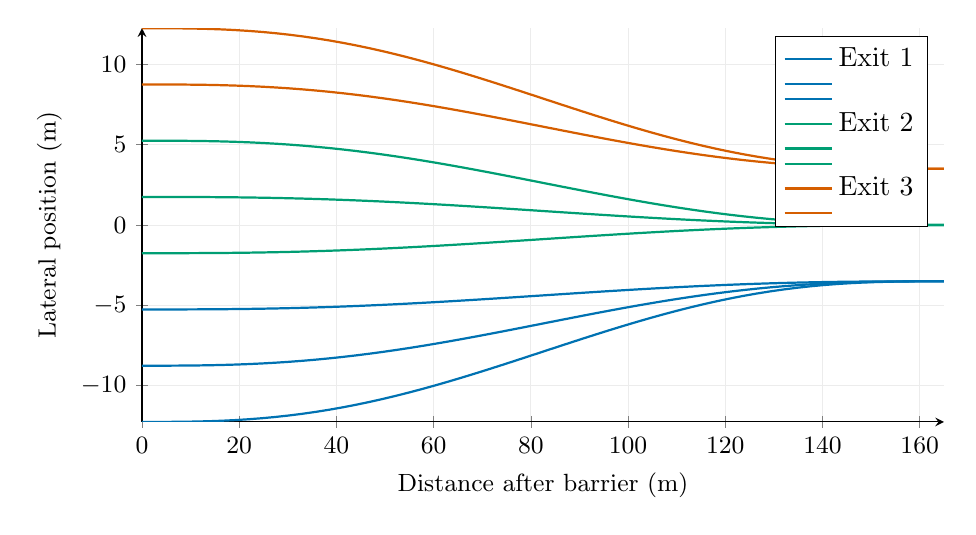
\begin{tikzpicture}\begin{axis}[width=.84\linewidth,height=5.0cm,scale only axis,xlabel={Distance after barrier (m)},ylabel={Lateral position (m)},axis lines=left,grid=major,grid style={gray!15},tick label style={font=\small},label style={font=\small}]\addplot[thick,main,no marks] coordinates {(0.0000,-12.25000) (2.7500,-12.24960) (5.5000,-12.24692) (8.2500,-12.23987) (11.0000,-12.22660) (13.7500,-12.20548) (16.5000,-12.17510) (19.2500,-12.13423) (22.0000,-12.08186) (24.7500,-12.01715) (27.5000,-11.93943) (30.2500,-11.84822) (33.0000,-11.74320) (35.7500,-11.62419) (38.5000,-11.49117) (41.2500,-11.34424) (44.0000,-11.18365) (46.7500,-11.00976) (49.5000,-10.82305) (52.2500,-10.62410) (55.0000,-10.41358) (57.7500,-10.19227) (60.5000,-9.96101) (63.2500,-9.72072) (66.0000,-9.47240) (68.7500,-9.21708) (71.5000,-8.95586) (74.2500,-8.68986) (77.0000,-8.42026) (79.7500,-8.14824) (82.5000,-7.87500) (85.2500,-7.60176) (88.0000,-7.32974) (90.7500,-7.06014) (93.5000,-6.79414) (96.2500,-6.53292) (99.0000,-6.27760) (101.7500,-6.02928) (104.5000,-5.78899) (107.2500,-5.55773) (110.0000,-5.33642) (112.7500,-5.12590) (115.5000,-4.92695) (118.2500,-4.74024) (121.0000,-4.56635) (123.7500,-4.40576) (126.5000,-4.25883) (129.2500,-4.12581) (132.0000,-4.00680) (134.7500,-3.90178) (137.5000,-3.81057) (140.2500,-3.73285) (143.0000,-3.66814) (145.7500,-3.61577) (148.5000,-3.57490) (151.2500,-3.54452) (154.0000,-3.52340) (156.7500,-3.51013) (159.5000,-3.50308) (162.2500,-3.50040) (165.0000,-3.50000)};\addlegendentry{Exit 1}\addplot[thick,main,no marks] coordinates {(0.0000,-8.75000) (2.7500,-8.74976) (5.5000,-8.74815) (8.2500,-8.74392) (11.0000,-8.73596) (13.7500,-8.72329) (16.5000,-8.70506) (19.2500,-8.68054) (22.0000,-8.64912) (24.7500,-8.61029) (27.5000,-8.56366) (30.2500,-8.50893) (33.0000,-8.44592) (35.7500,-8.37451) (38.5000,-8.29470) (41.2500,-8.20654) (44.0000,-8.11019) (46.7500,-8.00586) (49.5000,-7.89383) (52.2500,-7.77446) (55.0000,-7.64815) (57.7500,-7.51536) (60.5000,-7.37661) (63.2500,-7.23243) (66.0000,-7.08344) (68.7500,-6.93025) (71.5000,-6.77351) (74.2500,-6.61392) (77.0000,-6.45215) (79.7500,-6.28894) (82.5000,-6.12500) (85.2500,-5.96106) (88.0000,-5.79785) (90.7500,-5.63608) (93.5000,-5.47649) (96.2500,-5.31975) (99.0000,-5.16656) (101.7500,-5.01757) (104.5000,-4.87339) (107.2500,-4.73464) (110.0000,-4.60185) (112.7500,-4.47554) (115.5000,-4.35617) (118.2500,-4.24414) (121.0000,-4.13981) (123.7500,-4.04346) (126.5000,-3.95530) (129.2500,-3.87549) (132.0000,-3.80408) (134.7500,-3.74107) (137.5000,-3.68634) (140.2500,-3.63971) (143.0000,-3.60088) (145.7500,-3.56946) (148.5000,-3.54494) (151.2500,-3.52671) (154.0000,-3.51404) (156.7500,-3.50608) (159.5000,-3.50185) (162.2500,-3.50024) (165.0000,-3.50000)};\addlegendentry{}\addplot[thick,main,no marks] coordinates {(0.0000,-5.25000) (2.7500,-5.24992) (5.5000,-5.24938) (8.2500,-5.24797) (11.0000,-5.24532) (13.7500,-5.24110) (16.5000,-5.23502) (19.2500,-5.22685) (22.0000,-5.21637) (24.7500,-5.20343) (27.5000,-5.18789) (30.2500,-5.16964) (33.0000,-5.14864) (35.7500,-5.12484) (38.5000,-5.09823) (41.2500,-5.06885) (44.0000,-5.03673) (46.7500,-5.00195) (49.5000,-4.96461) (52.2500,-4.92482) (55.0000,-4.88272) (57.7500,-4.83845) (60.5000,-4.79220) (63.2500,-4.74414) (66.0000,-4.69448) (68.7500,-4.64342) (71.5000,-4.59117) (74.2500,-4.53797) (77.0000,-4.48405) (79.7500,-4.42965) (82.5000,-4.37500) (85.2500,-4.32035) (88.0000,-4.26595) (90.7500,-4.21203) (93.5000,-4.15883) (96.2500,-4.10658) (99.0000,-4.05552) (101.7500,-4.00586) (104.5000,-3.95780) (107.2500,-3.91155) (110.0000,-3.86728) (112.7500,-3.82518) (115.5000,-3.78539) (118.2500,-3.74805) (121.0000,-3.71327) (123.7500,-3.68115) (126.5000,-3.65177) (129.2500,-3.62516) (132.0000,-3.60136) (134.7500,-3.58036) (137.5000,-3.56211) (140.2500,-3.54657) (143.0000,-3.53363) (145.7500,-3.52315) (148.5000,-3.51498) (151.2500,-3.50890) (154.0000,-3.50468) (156.7500,-3.50203) (159.5000,-3.50062) (162.2500,-3.50008) (165.0000,-3.50000)};\addlegendentry{}\addplot[thick,green,no marks] coordinates {(0.0000,-1.75000) (2.7500,-1.74992) (5.5000,-1.74938) (8.2500,-1.74797) (11.0000,-1.74532) (13.7500,-1.74110) (16.5000,-1.73502) (19.2500,-1.72685) (22.0000,-1.71637) (24.7500,-1.70343) (27.5000,-1.68789) (30.2500,-1.66964) (33.0000,-1.64864) (35.7500,-1.62484) (38.5000,-1.59823) (41.2500,-1.56885) (44.0000,-1.53673) (46.7500,-1.50195) (49.5000,-1.46461) (52.2500,-1.42482) (55.0000,-1.38272) (57.7500,-1.33845) (60.5000,-1.29220) (63.2500,-1.24414) (66.0000,-1.19448) (68.7500,-1.14342) (71.5000,-1.09117) (74.2500,-1.03797) (77.0000,-0.98405) (79.7500,-0.92965) (82.5000,-0.87500) (85.2500,-0.82035) (88.0000,-0.76595) (90.7500,-0.71203) (93.5000,-0.65883) (96.2500,-0.60658) (99.0000,-0.55552) (101.7500,-0.50586) (104.5000,-0.45780) (107.2500,-0.41155) (110.0000,-0.36728) (112.7500,-0.32518) (115.5000,-0.28539) (118.2500,-0.24805) (121.0000,-0.21327) (123.7500,-0.18115) (126.5000,-0.15177) (129.2500,-0.12516) (132.0000,-0.10136) (134.7500,-0.08036) (137.5000,-0.06211) (140.2500,-0.04657) (143.0000,-0.03363) (145.7500,-0.02315) (148.5000,-0.01498) (151.2500,-0.00890) (154.0000,-0.00468) (156.7500,-0.00203) (159.5000,-0.00062) (162.2500,-0.00008) (165.0000,0.00000)};\addlegendentry{Exit 2}\addplot[thick,green,no marks] coordinates {(0.0000,1.75000) (2.7500,1.74992) (5.5000,1.74938) (8.2500,1.74797) (11.0000,1.74532) (13.7500,1.74110) (16.5000,1.73502) (19.2500,1.72685) (22.0000,1.71637) (24.7500,1.70343) (27.5000,1.68789) (30.2500,1.66964) (33.0000,1.64864) (35.7500,1.62484) (38.5000,1.59823) (41.2500,1.56885) (44.0000,1.53673) (46.7500,1.50195) (49.5000,1.46461) (52.2500,1.42482) (55.0000,1.38272) (57.7500,1.33845) (60.5000,1.29220) (63.2500,1.24414) (66.0000,1.19448) (68.7500,1.14342) (71.5000,1.09117) (74.2500,1.03797) (77.0000,0.98405) (79.7500,0.92965) (82.5000,0.87500) (85.2500,0.82035) (88.0000,0.76595) (90.7500,0.71203) (93.5000,0.65883) (96.2500,0.60658) (99.0000,0.55552) (101.7500,0.50586) (104.5000,0.45780) (107.2500,0.41155) (110.0000,0.36728) (112.7500,0.32518) (115.5000,0.28539) (118.2500,0.24805) (121.0000,0.21327) (123.7500,0.18115) (126.5000,0.15177) (129.2500,0.12516) (132.0000,0.10136) (134.7500,0.08036) (137.5000,0.06211) (140.2500,0.04657) (143.0000,0.03363) (145.7500,0.02315) (148.5000,0.01498) (151.2500,0.00890) (154.0000,0.00468) (156.7500,0.00203) (159.5000,0.00062) (162.2500,0.00008) (165.0000,0.00000)};\addlegendentry{}\addplot[thick,green,no marks] coordinates {(0.0000,5.25000) (2.7500,5.24976) (5.5000,5.24815) (8.2500,5.24392) (11.0000,5.23596) (13.7500,5.22329) (16.5000,5.20506) (19.2500,5.18054) (22.0000,5.14912) (24.7500,5.11029) (27.5000,5.06366) (30.2500,5.00893) (33.0000,4.94592) (35.7500,4.87451) (38.5000,4.79470) (41.2500,4.70654) (44.0000,4.61019) (46.7500,4.50586) (49.5000,4.39383) (52.2500,4.27446) (55.0000,4.14815) (57.7500,4.01536) (60.5000,3.87661) (63.2500,3.73243) (66.0000,3.58344) (68.7500,3.43025) (71.5000,3.27351) (74.2500,3.11392) (77.0000,2.95215) (79.7500,2.78894) (82.5000,2.62500) (85.2500,2.46106) (88.0000,2.29785) (90.7500,2.13608) (93.5000,1.97649) (96.2500,1.81975) (99.0000,1.66656) (101.7500,1.51757) (104.5000,1.37339) (107.2500,1.23464) (110.0000,1.10185) (112.7500,0.97554) (115.5000,0.85617) (118.2500,0.74414) (121.0000,0.63981) (123.7500,0.54346) (126.5000,0.45530) (129.2500,0.37549) (132.0000,0.30408) (134.7500,0.24107) (137.5000,0.18634) (140.2500,0.13971) (143.0000,0.10088) (145.7500,0.06946) (148.5000,0.04494) (151.2500,0.02671) (154.0000,0.01404) (156.7500,0.00608) (159.5000,0.00185) (162.2500,0.00024) (165.0000,0.00000)};\addlegendentry{}\addplot[thick,accent,no marks] coordinates {(0.0000,8.75000) (2.7500,8.74976) (5.5000,8.74815) (8.2500,8.74392) (11.0000,8.73596) (13.7500,8.72329) (16.5000,8.70506) (19.2500,8.68054) (22.0000,8.64912) (24.7500,8.61029) (27.5000,8.56366) (30.2500,8.50893) (33.0000,8.44592) (35.7500,8.37451) (38.5000,8.29470) (41.2500,8.20654) (44.0000,8.11019) (46.7500,8.00586) (49.5000,7.89383) (52.2500,7.77446) (55.0000,7.64815) (57.7500,7.51536) (60.5000,7.37661) (63.2500,7.23243) (66.0000,7.08344) (68.7500,6.93025) (71.5000,6.77351) (74.2500,6.61392) (77.0000,6.45215) (79.7500,6.28894) (82.5000,6.12500) (85.2500,5.96106) (88.0000,5.79785) (90.7500,5.63608) (93.5000,5.47649) (96.2500,5.31975) (99.0000,5.16656) (101.7500,5.01757) (104.5000,4.87339) (107.2500,4.73464) (110.0000,4.60185) (112.7500,4.47554) (115.5000,4.35617) (118.2500,4.24414) (121.0000,4.13981) (123.7500,4.04346) (126.5000,3.95530) (129.2500,3.87549) (132.0000,3.80408) (134.7500,3.74107) (137.5000,3.68634) (140.2500,3.63971) (143.0000,3.60088) (145.7500,3.56946) (148.5000,3.54494) (151.2500,3.52671) (154.0000,3.51404) (156.7500,3.50608) (159.5000,3.50185) (162.2500,3.50024) (165.0000,3.50000)};\addlegendentry{Exit 3}\addplot[thick,accent,no marks] coordinates {(0.0000,12.25000) (2.7500,12.24960) (5.5000,12.24692) (8.2500,12.23987) (11.0000,12.22660) (13.7500,12.20548) (16.5000,12.17510) (19.2500,12.13423) (22.0000,12.08186) (24.7500,12.01715) (27.5000,11.93943) (30.2500,11.84822) (33.0000,11.74320) (35.7500,11.62419) (38.5000,11.49117) (41.2500,11.34424) (44.0000,11.18365) (46.7500,11.00976) (49.5000,10.82305) (52.2500,10.62410) (55.0000,10.41358) (57.7500,10.19227) (60.5000,9.96101) (63.2500,9.72072) (66.0000,9.47240) (68.7500,9.21708) (71.5000,8.95586) (74.2500,8.68986) (77.0000,8.42026) (79.7500,8.14824) (82.5000,7.87500) (85.2500,7.60176) (88.0000,7.32974) (90.7500,7.06014) (93.5000,6.79414) (96.2500,6.53292) (99.0000,6.27760) (101.7500,6.02928) (104.5000,5.78899) (107.2500,5.55773) (110.0000,5.33642) (112.7500,5.12590) (115.5000,4.92695) (118.2500,4.74024) (121.0000,4.56635) (123.7500,4.40576) (126.5000,4.25883) (129.2500,4.12581) (132.0000,4.00680) (134.7500,3.90178) (137.5000,3.81057) (140.2500,3.73285) (143.0000,3.66814) (145.7500,3.61577) (148.5000,3.57490) (151.2500,3.54452) (154.0000,3.52340) (156.7500,3.51013) (159.5000,3.50308) (162.2500,3.50040) (165.0000,3.50000)};\addlegendentry{}\end{axis}\end{tikzpicture}\caption{Order-preserving centerline paths for the selected baseline. Curves within one group merge at its assigned exit. Release spacing is a separate control requirement.}\label{fig:paths}\end{figure}
\section{Recommendation}
Do not build or operate to the pooled capacity estimate. Staffed service is the first bottleneck to investigate. A payment-aware allocation, compared under light and heavy traffic and checked against finite storage, is needed before choosing a preferred layout. The smooth taper gives an explicit geometric starting point, while its safety interpretation remains limited to the stated kinematics.
\clearpage\section*{Letter to the New Jersey Turnpike Authority}
\addcontentsline{toc}{section}{Letter to the New Jersey Turnpike Authority}
\noindent Dear Members of the Authority,

We recommend treating a toll plaza as a set of payment-compatible services connected to receiving traffic lanes. The number of open booths by itself can be misleading: unused electronic capacity cannot process a driver who requires a staffed booth. The operating plan should identify the limiting payment or exit group before adding pavement or changing discharge speeds.
Our initial calculation finds that the pooled 5,400-vehicle/hour figure overstates what the current payment mix can use. The staffed-booth restriction gives only 3,000 vehicles per hour for the baseline arrangement. Heavy demand of 3,600 vehicles per hour therefore cannot be accommodated indefinitely. More favorable exit headways alone do not remove this payment bottleneck.
We propose a smooth, channelized fan-in and payment-aware allocation as the next design step. We have not yet quantified finite queues or established the preferred booth mix; a construction commitment should wait for that comparison and local measurements.
Before construction, measure payment proportions and service times, test route-guidance compliance, and check finite holding space and vehicle trajectories. Our idealized centerlines and release intervals address specific kinematic concerns, but do not estimate crashes or replace engineering standards. A pilot can first change signs and booth assignments; major pavement expansion should follow only when the observed limiting mechanism justifies it.
\noindent Respectfully,\\Team 7391857
\clearpage
\begin{thebibliography}{9}
\bibitem{comap} COMAP. 2017 MCM Problem B: Merge After Toll. 2017. Official problem statement.
\url{https://www.contest.comap.com/undergraduate/contests/mcm/contests/2017/problems/2017_MCM_Problem_B.pdf}.
\bibitem{fhwa} Federal Highway Administration. Traffic Analysis Toolbox, Volume III: Guidelines for Applying Traffic Microsimulation Modeling Software. 2004, Chapter 5, Model Calibration. FHWA-HRT-04-040.
\url{https://ops.fhwa.dot.gov/trafficanalysistools/tat_vol3/sect5.htm}.
\end{thebibliography}
\clearpage\section*{Report on Use of AI Tools}
\addcontentsline{toc}{section}{Report on Use of AI Tools}
An OpenAI Codex agent conducted the problem interpretation, mathematical modeling, programming, numerical experiments and English writing in one delegated research episode. The agent selected the historical task and read its official statement and general FHWA guidance. No same-problem submitted solution or judges' commentary was consulted during this episode. Possible exposure during model pretraining is unknown.

The user supplied the plugin-development objective and authorized local research; the user did not supply this case's model choices or perform its mathematical verification. Other agent roles of the same model family reviewed the numerical tools and, where recorded in the accompanying archive, the case. Such review is not human verification or independent field validation.

Python and its scientific libraries performed layout enumeration, flow construction and queue calculations. LaTeX produced this document. Numerical verification checks the model against distinct algorithms and analytic conditions; it does not establish empirical safety or traffic calibration. The accompanying research archive retains the available run receipts, failed candidates and review scope. Full raw model input/output transcripts are not available in that archive, and no complete interaction log is reconstructed from summaries.
\end{document}

